\part{Análisis de requerimientos}\label{part:analisis}
\section{Requerimientos}
\subsection{Funcionales}
\begin{itemize}
	\item La aplicación de PC deberá ser capaz de poder iniciar una conexión segura con el sistema utilizando la misma para enviar los mensajes que el cliente desee.
	\item La aplicación podrá enviar peticiones de forma de obtener el mensaje actual del cartel o incluso establecer uno nuevo. Por otra parte, también podrá pedir los datos de la red a la que el sistema estará conectado o cambiarlos.
	\item La aplicación deberá ser capaz de modificar parámetros de animación tales como frecuencia de parpadeo y velocidad de desplazamiento lateral o estaticidad.
	\item La aplicación deberá poder recuperar los valores actuales de los parámetros de animación que posee el cartel.
	\item La aplicación permitirá al usuario, ingresar por teclado el mensaje que desea mostrar mediante los caracteres que se establecen en el estándar de codificación de caracteres ISO/IEC 8859-1 (ver \cite{CodifChar}).
	\item El cartel deberá poder procesar sólo mensajes a través del protocolo diseñado específicamente para este proyecto (ver sección \ref{sec:protocolo}).
	\item El cartel deberá mostrar los mensajes que desee el usuario de forma legible.
	\item Tanto el cartel como la aplicación de PC deberán ser capaces de conectarse a una red WiFi que el cliente desee.
	\item El cartel deberá poder almacenar y modificar sus credenciales de red de forma de poder conectarse al WiFi que el cliente desee.
	\item El cartel deberá obtener una contraseña de acceso al sistema para realizar cualquier operación mencionada anteriormente.
	\item El cartel deberá mantener los datos de configuración y del mensaje que muestra, aún cuando el mismo haya sido desconectado de la red inalámbrica o de la red eléctrica.
	\item El cartel deberá poder pasar a un estado por defecto en cuanto a credenciales de red, mensaje y parámetros de animación cuando el sistema se resetea manualmente o cuando el mismo se quede en un estado incorrecto.
	\item El hardware del cartel debe poder escalar la cantidad de módulos de LEDs.
	\item El hardware del cartel debe permitir indicar la cantidad de módulos de LEDs conectados, de manera tal que el programa del microcontrolador sepa con cuántos de ellos está operando en todo momento.
	\item El sistema que controla el cartel debe estar preparado para escalar en caso de que se agreguen más módulos de LEDs.
	%TODO AMG - Requerimientos de hardware??
\end{itemize}

\subsection{No funcionales}
\begin{itemize}
	\item El tiempo de respuesta del cartel no debe exceder los cinco segundos.
	\item El sistema entero no debe consumir mas de 30 Watts bajo operación normal.
	\item El sistema deberá ser capaz de aceptar sólo conexiones por TLS \cite{TLS} de forma que las conexiones y el intercambio de paquetes sea cifrado y seguro.
	%TODO AMG - Si podemos meter algunos requerimientos no funcionales más, joya!
\end{itemize}

\subsection{Interacción con el usuario}
	
	Se denomina usuario del sistema a toda persona con acceso autorizado a su configuración y puesta en marcha.	El usuario tendrá la posibilidad de agregar o quitar módulos esclavos al cartel con el fin de proveerle mayor longitud, de acceder al panel de configuración del cartel para modificar su mensaje y características del mismo.
	
	Para operar correctamente el cartel, únicamente es necesario que el usuario tenga a su disposición una PC, en la cual utilizará un aplicativo desarrollado con una interfaz gráfica para controlar el cartel. Para realizar la instalación del sistema, se requiere solamente al manual de instalación (ver \ref{sec:inst-hw}).

	No es necesario que el usuario tenga conocimientos de programación.
	Sin embargo, una noción básica de electrónica es deseable para evitar que algún componente o conexión eléctrica del sistema se vea perjudicada durante su instalación.
	
	A la hora de añadir y eliminar módulos esclavos, es necesario actualizar la información en el programa de forma de hacerle conocer al sistema, que la cantidad de módulos ha sido modificada. Esto se realiza conectando y desconectando jumpers que se encuentran en el módulo maestro del cartel.
	El usuario debe poseer un conocimiento básico de esta operación para poder realizarla satisfactoriamente.
	
	

\section{Especificaciones físicas}

	El sistema está conformado por módulos de dos tipos claramente distinguibles: un módulo maestro y módulos esclavos.

	El módulo maestro, que se caracteriza por tener la ficha de alimentación y no estar conectada a una matriz de LEDs, se encarga de controlar la cadena de módulos esclavos. Sólo un módulo de este tipo es necesario por cartel.
	Adicionalmente este componente posee un microcontrolador que gobierna la totalidad del sistema y un conjunto de jumpers que permiten establecer la cantidad de módulos esclavos con los que se operará.
	Por último esté módulo, posee un botón de reset que permite enviar al sistema a un estado conocido, ya sea ante un fallo o incluso, ante un cambio en alguno de los valores relacionados a sus credenciales de red.

	Por otro lado, están los módulos esclavos, que se encargan de controlar su matriz de LEDs para representar un mapa de bits y de funcionar como eslabón en la cadena de módulos esclavos. Se puede ver en la figura \ref{fig:dibujo-real} un dibujo ilustrativo exhibiendo los componentes más relevantes del sistema.
	\begin{description}
		\item[A: ] Fuente de alimentación (AC 220V a 5V DC).
		\item[B: ] Cables de interconexión maestro-esclavo y esclavo-esclavo.
		\item[C: ] Módulo esclavo.
		\item[D: ] Módulo maestro.
		\item[E: ] Cables de conexión a la matriz de LEDs.
		\item[F: ] Matriz de LEDs.
		\item[G: ] Pulsador de reset.
		\item[H: ] Jumpers de configuración.
		\item[I: ] NodeMCU ESP-12
		\item[J: ] MAX7219.
	\end{description}
	
	\begin{figure}[ht!]
		\begin{center}
			\centering
			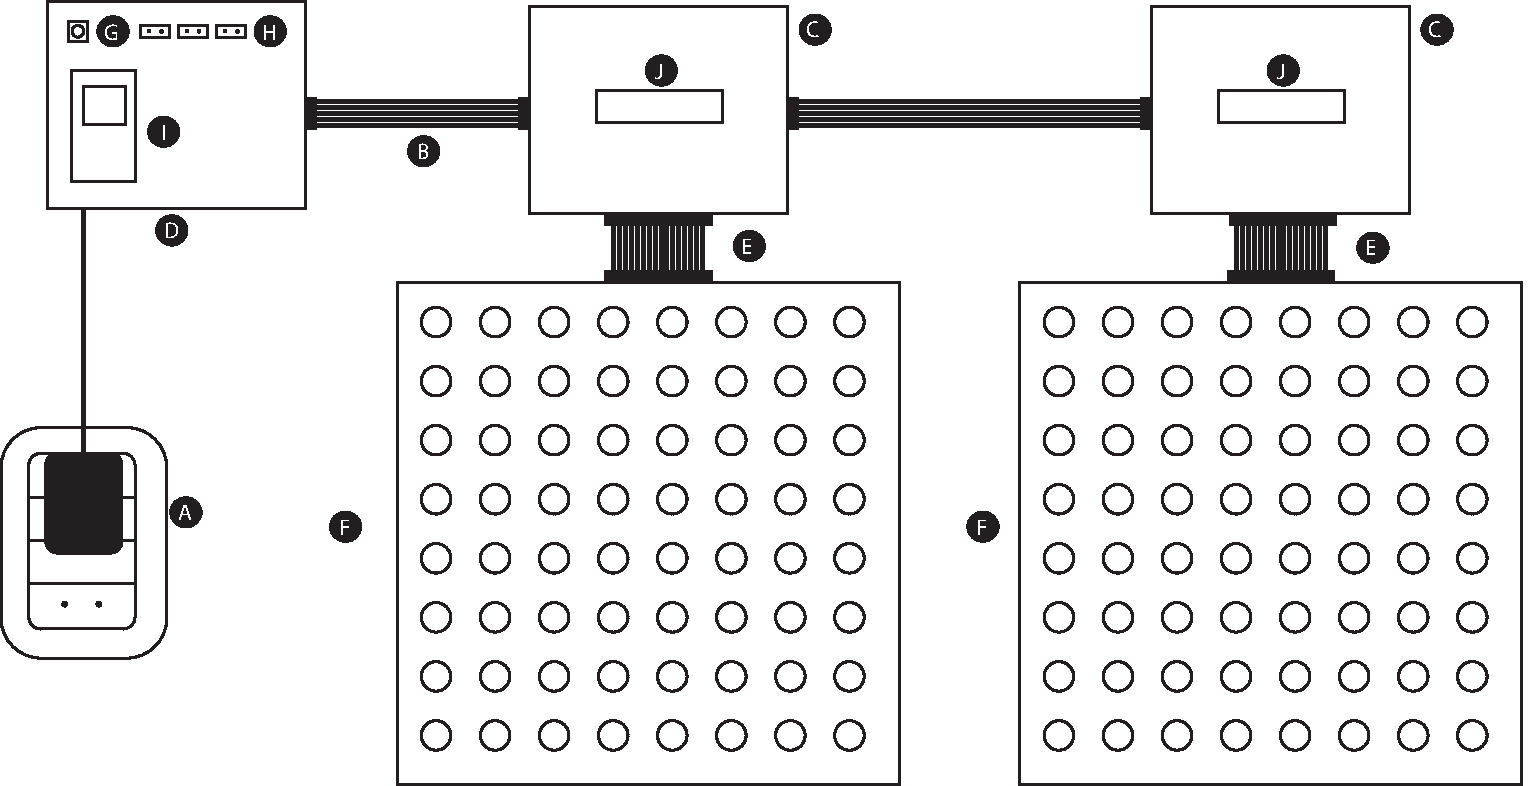
\includegraphics[width=\linewidth]{imagenes/dibujo-fisico.pdf}
			\caption{Dibujo ilustrativo del hardware del sistema.}
			\label{fig:dibujo-real}
		\end{center}
	\end{figure}


\section{Cronograma de actividades}
%TODO AMG - Se debe agregar una breve descripción de las actividades y la foto del cronograma.


\section{Componentes de hardware}
A la hora de construir el cartel, se debe armar tanto un módulo maestro y uno o más módulos esclavos, siendo éstos últimos los encargados de mostrar los mensajes en el cartel.
En el apéndice \ref{sec:materiales} se listan los componentes de cada módulo y las herramientas necesarias para la construcción de los mismos.


\section{Estimación de costos}
Como se explicó en la sección anterior, en todo proyecto es necesario realizar tanto una estimación del tiempo de desarrollo del sistema como una aproximación a los costos que tendrá el mismo.
Por dicho motivo, en el apéndice \ref{sec:presupuesto} se detalla el valor aproximado que posee cada material listado previamente.